\documentclass[tikz,border=3pt]{standalone}
\usepackage[utf8]{inputenc}
\usepackage[T1]{fontenc}
\usepackage{lmodern}
\renewcommand{\familydefault}{\sfdefault}
\usepackage{sansmath}\sansmath
\usepackage{chemfig}
\usepackage{pgfplots}\pgfplotsset{compat=1.18,/pgf/number format/use comma,/pgf/number format/1000 sep={.}}
\usetikzlibrary{arrows.meta,calc,positioning,decorations.pathmorphing,patterns}
% paleta del sitio
\definecolor{nar}{HTML}{E8680C}\definecolor{narc}{HTML}{FFB35C}\definecolor{hielo}{HTML}{FFF3E8}
\definecolor{tinta}{HTML}{1D1D1F}\definecolor{gris}{HTML}{6E6E73}\definecolor{lila}{HTML}{7C5CF0}
\definecolor{azul}{HTML}{2F6FD6}\definecolor{menta}{HTML}{17A673}\definecolor{coral}{HTML}{E8342A}
\begin{document}
% escala: 1 cm de la regla = 0,12 unidades del dibujo; el 0 de la regla está en y = 0
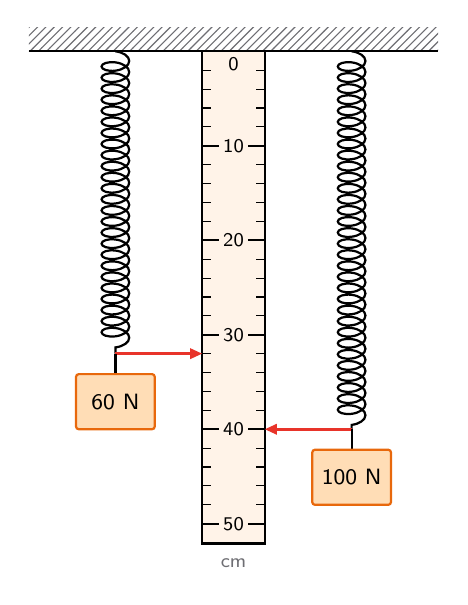
\begin{tikzpicture}[font=\footnotesize,>={Stealth[length=2mm]}]
\fill[pattern=north east lines,pattern color=gris] (-2.6,0) rectangle (2.6,0.3);
\draw[thick] (-2.6,0) -- (2.6,0);
% regla
\draw[thick,fill=hielo] (-0.4,0) rectangle (0.4,-6.25);
\foreach \c in {0,2,...,50} \draw (-0.4,-0.12*\c) -- (-0.28,-0.12*\c) (0.4,-0.12*\c) -- (0.28,-0.12*\c);
\foreach \c in {0,10,...,50} {\draw[thick] (-0.4,-0.12*\c) -- (-0.18,-0.12*\c) (0.4,-0.12*\c) -- (0.18,-0.12*\c);
  \ifnum\c>0 \node[font=\scriptsize,fill=hielo,inner sep=1pt] at (0,-0.12*\c) {\c};\fi}
\node[font=\scriptsize] at (0,-0.16) {0};
\node[gris,font=\scriptsize] at (0,-6.5) {cm};
% resorte 1: 60 N, puntero en 32 cm
\draw[thick,decorate,decoration={coil,aspect=0.5,segment length=4pt,amplitude=5pt}] (-1.5,0) -- (-1.5,-3.84);
\draw[very thick,coral] (-1.5,-3.84) -- (-0.45,-3.84);
\fill[coral] (-0.4,-3.84) -- (-0.55,-3.77) -- (-0.55,-3.91) -- cycle;
\draw[thick] (-1.5,-3.84) -- (-1.5,-4.1);
\draw[thick,draw=nar,fill=narc!45,rounded corners=1pt] (-2.0,-4.1) rectangle (-1.0,-4.8);
\node at (-1.5,-4.45) {60 N};
% resorte 2: 100 N, puntero en 40 cm
\draw[thick,decorate,decoration={coil,aspect=0.5,segment length=4pt,amplitude=5pt}] (1.5,0) -- (1.5,-4.8);
\draw[very thick,coral] (1.5,-4.8) -- (0.45,-4.8);
\fill[coral] (0.4,-4.8) -- (0.55,-4.73) -- (0.55,-4.87) -- cycle;
\draw[thick] (1.5,-4.8) -- (1.5,-5.06);
\draw[thick,draw=nar,fill=narc!45,rounded corners=1pt] (1.0,-5.06) rectangle (2.0,-5.76);
\node at (1.5,-5.41) {100 N};
\end{tikzpicture}
\end{document}
